\documentclass{article}

\usepackage{graphicx}
\usepackage{amsmath} 
\usepackage{float}

\usepackage{xepersian}
\settextfont{B Nazanin}


\begin{document}

\section{\lr{OFDM } نوری}

یکی از حوزه های جذاب انتقال اطلاعات استفاده از نور و ادوات نوری همچون \lr	 {LED}ها و لیزر ها برای انجام این کار است. یکی از معضلاتی که ما در ارسال اطلاعات داریم تخصیص پهنای باند است و روز به روز با توجه به گسترده شدن دستگاه های هوشمند و  موبایل ها به این مشکل افزوده میشود، این روش باعث میشود که معضل تخصیص پهنای باند را فراموش کنیم و به انتقال اطلاعات بپردازیم. از جمله تفاوت هایی که این شیوه انتقال اطلاعات با روش های کلاسیک و مدرن دارد این است که ما نمیتوانیم از روش های مدولاسیون های مرسوم و مدولاسیون های تک حامل استفاده کنیم، از دلایل این امر میتوان به این نکته اشاره کرد که به دلیل تفاوت نحوه ارسال اطلاعات ( ارسال با شدت نور) امکان تداخل بین نمونه ها افزایش پیدا مبکند و علی الخصوص این امر در ارسال اطلاعات با نرخ بیت بالا خود را نشان میدهد و همچنین در ارسال اطلاعات استفاده از مدولاسیون های تک حامل باعث میشود که نتوانیم این ویژگی را به سیستم دهیم که چند کاربر بطور همزمان بتوانند به ارسال و دریافت اطلاعات بپردازند. در نتیجه رو به استفاده از مدولاسیون \lr{OFDM} می آوریم.
همان طور که مشخص است ما باز هم در استفاده از مدولاسیون \lr{OFDM} برای کاربرد نوری  با چالش روبرو میشویم چرا که در \lr{OFDM} مرسوم ما بیت هایی مختلط را ارسال میکنیم ولی در این سیستم مخابراتی نوری اطلاعات با شدت نور ارسال میشوند ، پس واضح است که نمیتوانیم از عددی مختلط به شدت نور برسیم. چالش دیگر هم این است که ما باز هم نمیتوانیم عددی منفی را به عنوان شدت نور لیزر در نظر بگیریم. دلایل ذکر شده مشخص میکند که ما برای انجام این مهم باید تغییراتی در سیستم \lr{OFDM} مرسوم و معمولی به وجود بیاوریم. 
از جمله مهم ترین روش های در \lr{OFDM} نوری میتوان به \lr{ACO-OFDM}  و \lr{DCO-OFDM} اشاره کرد. تفاوت دو روش یاد شده در برطرف کردن چالش های ذکر شده است. این تفاوت در روش باعث میشود که در موارد مختلف بر حسب کاربرد از کدام روش استفاده کنیم.

\subsection{\lr{ACO-OFDM}}


در \lr{ACO-OFDM}       \LTRfootnote{Asymmetrically Clipped Optical}
تنها زیر حامل های با اندیس فرد اطلاعات را انتقال میدهند. در حالی که زیر حامل های با اندیس زوج یک بایاس را ایجاد میکنند که باعث میشوند  سیگنال \lr{OFDM} ارسال شده بتواند غیر منفی شود.\cite{2}
\begin{figure}[h!]
\begin{center}
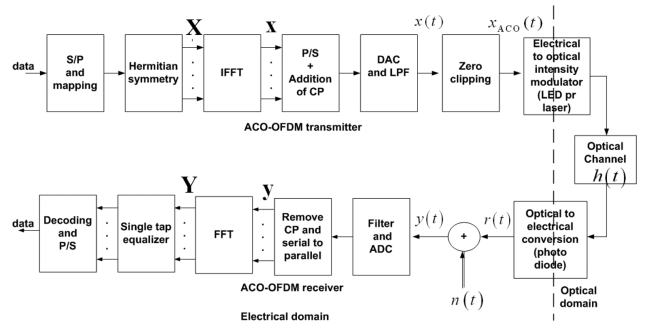
\includegraphics[width=9cm, height=4cm]{aco.PNG}
\end{center}
\caption{  سیستم \lr{ACO-OFDM}}
\label{acomodel}

\end{figure}
\ \newpage

\subsubsection{فرستنده و گیرنده }
 شکل \ref{acomodel} یک سیستم \lr{ACO-OFDM} را نشان میدهد. سیگنال ورودی به \lr{,\textbf{X},IFFT} تنها از اندیس های فرد تشکیل شده و اندیس های زوج برابر صفر قرار گرفته اند.\lr{\textbf{X}$ = [0,X_{1},0,X_{3},....,X_{N-1}]$} ‌همچنین وکتور  \lr{\textbf{X}} دارای تقارن هرمیتی  \LTRfootnote{hermitian symmetry} میباشد چرا که میخواهیم وکتور خروجی  \lr{,\textbf{x},IFFT}  حقیقی باشد. در شکل \ref{acovec} بردار ورودی به  \lr{IFFT} مشخص شده است.\cite{1} سیگنال خروجی  \lr{,\textbf{x},}  حقیقی میباشد و دارای ویژگی ضد تقارن \LTRfootnote{anti symmetry} است  همانطور که در رابطه زیر میبینیم.\cite{6}
برای واضح تر شدن این موضوع شبیه سازی انجام شده در متلب برای خروجی  \lr{,\textbf{x},IFFT} در شکل\ref{aco} آمده است و مشاهده میشود که با تساوی \ref{acoanti} همخوانی دارد.
\begin{equation}
x_{k} = -x_{k+\frac{N}{2}}    \hspace{8pt}\textrm{\lr{for}}  \hspace{4pt}  0 < k < \frac{N}{2} .
\label{acoanti}
\end{equation}


\begin{figure}[H]
\begin{center}
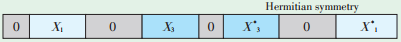
\includegraphics[width=9cm]{vec.PNG}
\end{center}
\caption{ورودی \lr{IFFT} در \lr{ACO-OFDM}}
\label{acovec}
\end{figure}



\begin{figure}[H]
\begin{center}
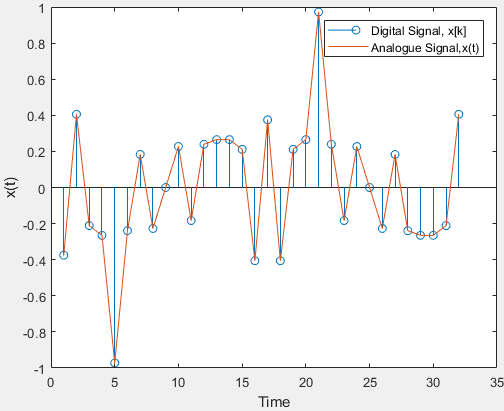
\includegraphics[width=9cm]{xaco.PNG}
\end{center}
\caption{خروجی  \lr{\textbf{x},IFFT} در\lr{ACO-OFDM}    }
\label{aco}
\end{figure}


فرستنده \lr{ACO-OFDM} خیلی شبیه به \lr{DCO-OFDM} است. ابتدا \lr{x} سریال میشود و سپس \lr{CP} \LTRfootnote{Cyclic Perfix} را انجام میدهیم.  \lr{x}  به آنالوگ تبدل میشود و خروجی از یک فیلتر پایین گذر ایده آل عبور میکند و نتیجه$ x(t)‌$ میشود. به دلیل این که نمونه های منفی نمیتوانند ارسال شوند چون سیستم \lr{IM/DD} است. در صفر قطع میشود و سیگنال \lr{ $x_{ACO}(t)$, ACO-OFDM} حاصل میشود در شکل \ref{acoclipped} میتواند این سیگنال را مشاهده کنید . بخاطر خاصیت ضد تقارن این سیگنال که در رابطه \ref{acoanti}  مشاهده شد با بریدن و قطع کردن سیگنال در صفر هیچ اطلاعاتی از بین نمی رود. هم چنین با بریدن و قطع کردن سیگنال یک نویز جدید مانند تداخل روی زیرحامل های زوج به وجود می آید.\cite{4} سپس  \lr{ $x_{ACO}(t)$} به عنوان ورودی به فرستنده نوری ایده آل داده می شود و ساختار گیرنده هم دقیقا مانند گیرنده \lr{DCO-OFDM}  است با این تفاوت که در \lr{ACO-OFDM} ‌ تنها زیر حامل های فرد دمودله میشوند چرا که تنها این زیر حامل ها اطلاعات را انتقال می دهند.

\begin{figure}[H]
\begin{center}
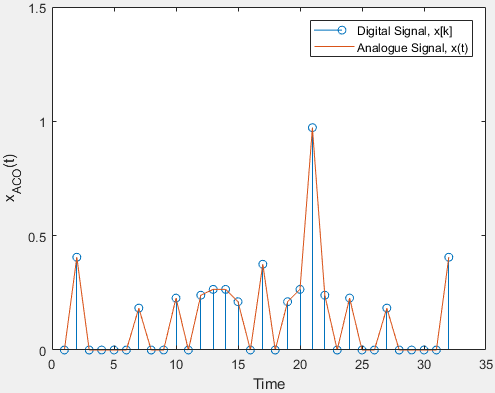
\includegraphics[width=9cm]{xacoclipped.PNG}
\end{center}
\caption{ \lr{ $x_{ACO}(t)$}  }
\label{acoclipped}
\end{figure}

\subsubsection{محاسبه احتمال خطا}
در این قسمت احتمال خطا \lr{ACO-OFDM} مورد بررسی قرار میگیرد و فرمول تئوری بدست آمده از مقاله فلان همراه با شبیه سازی سیستم در یک نمودار نشان داده میشوند. فرمول احتمال خطای \lr{ACO-OFDM} در زیر آمده است.

\begin{equation}
BER_{ACO} = \frac{2(\sqrt{M}-1)}{\sqrt{M}\times \log_{2}\sqrt{M}} \times Q(\sqrt{\frac{3\times SNR}{M - 1}})
\label{acober}
\end{equation}


در نمودار زیر نیز هم نمودار های تئوری و هم نمودارهای حاصل از شبیه سازی رسم شده اند.

\begin{figure}[H]
\begin{center}
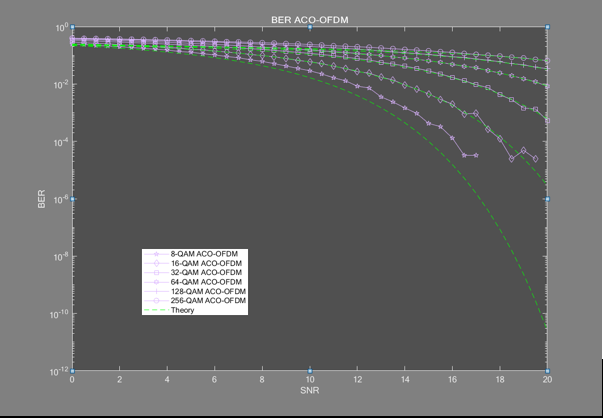
\includegraphics[width=12cm, height=9cm]{acober.PNG}
\end{center}
\caption{احتمال خطا سیستم \lr{ACO-OFDM}}
\label{acomod}

\end{figure}













\section{\lr{DCO-OFDM}}
روش دیگری که در \lr{Optical-OFDM}\ در سیستم های مخابرات نوری استفاده می شود روش \lr{DCO- OFDM}       \LTRfootnote{DC biased optical OFDM}
می باشد.\lr{OFDM}\ معمولی در انتها یک سیگنال مختلط ایجاد می‌کند اما چون در سیستم های مخابراتی نوری از \lr{LED} \LTRfootnote{Light Emitting Diode} استفاده می شود و \lr{LED} نیز فقط قادر به مدوله کردن شدت نور می باشد، بنابراین سیگنالی که ایجاد می شود باید حقیقی و مثبت باشد. 

\begin{figure}[h!]
\begin{center}
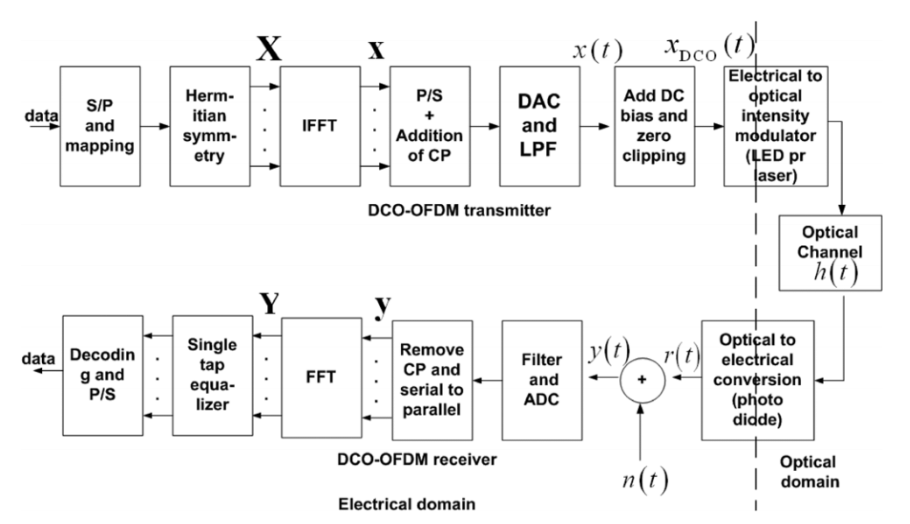
\includegraphics[width=9cm, height=5cm]{dco.PNG}
\end{center}
\caption{  سیستم \lr{DCO-OFDM}}
\label{dcomodel}

\end{figure}
\subsection{فرستنده و گیرنده}
خروجی سیستم \lr{IFFT}\ مطابق با رابطه‌ی زیر به دست می‌آید:
\begin{equation}
x_{m} = \frac{1}{N}\sum_{m=0}^{N-1}X_{k}e^{j \frac{2 \pi km}{N}}    \hspace{8pt}\textrm{\lr{for}}  \hspace{4pt}  0 \leq m \leq N-1 .
\label{dcoanti}
\end{equation}

در تکنیک \lr{DCO-OFDM}\ بردار \lr{X}\ را به گونه ای در نظر می‌گیرند که خروجی رابطه‌ی  \ref{dcoanti} یک سیگنال حقیقی بشود.
\begin{equation}
X=[X_{1},X_{2},X_{3},...,X_{N-1}]
\label{ofdmseq}
\end{equation}
\begin{equation}
X_{DCO}=[0,X_{1},X_{2},X_{3},...,X_{N-1},0,X_{N-1}^{*},X_{N-2}^{*},X_{N-3}^{*},...,X_{1}^{*}]
\label{dcoseq}
\end{equation}

در این صورت طول \lr{X}\ برابر با \lr{2N} می‌شود و رابطه‌ \lr{IFFT}\ برای \lr{X}\ را به صورت زیر می‌توان نوشت:
\begin{equation}
x_{m} = \frac{1}{N}\sum_{m=0}^{2N-1}X_{k}e^{j \frac{2 \pi km}{N}}    \hspace{8pt}\textrm{\lr{for}}  \hspace{4pt}  0 \leq m \leq 2N-1 .
\label{dcoifft}
\end{equation}
تا اینجا با استفاده از تکرار کردن اطلاعات و از دست دادن بهره‌ی طیفی سیگنال حقیقی به دست آمده است.اما در مرحله‌ی بعدی طبق شکل \ref{dcomodel}\ اضافه کردن  \lr{Cyclic Prefix}\ می‌باشد. در این بلوک اگر طول رشته‌ی ورودی \lr{L}\ باشد، به تعداد \lr{L/4}\ از انتهای رشته را در ابتدای رشته‌ی ورودی کپی می‌کنیم. این کار باعث می‌شود که گیرنده دچار \lr{ISI} \LTRfootnote{Inter Symbol interference}\ نشود.

در مرحله‌ی بعدی که اصلی ترین قسمت روش \lr{DCO-OFDM} می‌باشد، برای ایجاد یک سیگنال حقیقی و مثبت باید مقادیر منفی سیگنال را به مقادیر مثبت تبدیل کرد. بنابراین یک مقدار \lr{DC} به سیگنال افزوده می‌شود. این مقدار بایاس طبق شکل \ref{dcomodel}\ در حالت پیوسته به سیگنال افزوده می‌شود.
\begin{equation}
x_{DCO}(t)=x(t)+B_{DC} \hspace{8pt}
\label{dcox}
\end{equation}

بعد از این مراحل سیگنال دیگر تغییری پیدا نمی‌کند و درگیرنده ابتدا با فرض سنکرون بودن گیرنده و فرستنده قسمت \lr{Cyclic Prefix}\ حذف می‌شود.پس از آن از حوزه‌ی زمان با استفاده از ماژول \lr{FFT}\ به حوزه‌فرکانس بازمی گردد.

\lr{Single Tap Equalizer} نیز برای حذف اثرات کانال می‌باشد. دراین قسمت در ضمن می توان اثراتی هم چون \lr{Multi-Path fading} را نیز کم کرد و پس از حذف اثرات کانال مطابق با آن مدلاسیونی که در فرستنده استفاده شده است، دمدولاسیون انجام می‌شود و سیگنال اطلاعات به دست می‌آید.  

یکی از معایب این روش مصرف انرژی زیاد می‌باشد و از لحاظ انرژی خیلی بهینه نمی باشد، زیرا که در فرستنده با افزودن بایاس به سیگنال انرژی سیگنال زیاد می‌شود و هم چنین با افزودن سیگنال بایاس به سیگنال اصلی احتمال اشباع شدن بیشتر می‌شود.


\subsection{شبیه سازی}
در این قسمت شبیه سازی این روش در متلب انجام شده است و نمودار \lr{Bit Error Rate}\ را به دست آورده‌ایم. در ابتدا سیگنال تصادفی‌ای را به عنوان 

\clearpage
\setLTRbibitems
\begin{thebibliography}{9}
\resetlatinfont
\bibitem{2}
J. Armstrong and B. J. C. Schmidt, “Comparison of asymmetrically
clipped optical OFDM and DC-biased optical OFDM in AWGN,”
IEEE Commun. Lett., vol. 12, pp. 343–345, 2008.
\bibitem{1}
H. Elgala, R. Mesleh, and H. Haas, “Practical considerations for indoor wireless optical system implementation using OFDM,” in Pro.
ConTEL, Zagreb, Croatia, 2009, pp. 25–30.
\bibitem{4}
J. Armstrong and A. J. Lowery, “Power efficient optical OFDM,” Electron. Lett., vol. 42, pp. 370–372, 2006.
\bibitem{6}
K. Asadzadeh, A. Dabbo, and S. Hranilovic, “Receiver design for
asymmetrically clipped optical OFDM,” in Proc. IEEE GLOBECOM
OWC Workshop, Houston, TX, USA, 2011.
\end{thebibliography}


\end{document}

